\documentclass[usegraphicx,usenatbib]{mn2e}

%\usepackage[letterpaper]{geometry}
%\usepackage{draftwatermark}

\usepackage{graphicx}
\usepackage{verbatim}
\usepackage{color}
\usepackage{xcolor}
\usepackage[normalem]{ulem} % for striking out with \sout
\usepackage{amsmath} % for boldsymbol
\usepackage{times}
\usepackage{mathabx}
\usepackage{enumitem}

% A comment block

%\newcommand{\comment}[1]{}

% For color
\newcommand{\mpname}[1]{#1_color.eps}
\newcommand{\clraitoff}{red}
\newcommand{\lumblack}{(black)}
\newcommand{\lumblue}{(blue)}
\newcommand{\lumred}{(red)}
\newcommand{\vdisred}{(red-dashed curve)}
\newcommand{\vdisblue}{(blue-solid curve)}

% For bw
%\newcommand{\mpname}[1]{#1.eps}
%\newcommand{\clraitoff}{}
%\newcommand{\lumblack}{}
%\newcommand{\lumblue}{}
%\newcommand{\lumred}{}
%\newcommand{\vdisred}{(dashed curve)}
%\newcommand{\vdisblue}{(solid curve)}

\newcommand{\umag}{$u$}
\newcommand{\gmag}{$g$}
\newcommand{\rmag}{$r$}
\newcommand{\imag}{$i$}
\newcommand{\zmag}{$z$}
\newcommand{\gmr}{$g-r$}



\newcommand{\gammat}{$\gamma_T$}
\newcommand{\gammacross}{$\gamma_\times$}
\newcommand{\deltasig}{$\Delta \Sigma$}
\newcommand{\deltaplus}{$\Delta \Sigma_+$}
\newcommand{\deltacross}{$\Delta \Sigma_\times$}
\newcommand{\deltarho}{$\Delta \rho$}
\newcommand{\movr}{$M(<r)$}
\newcommand{\sigmacrit}{$\Sigma_{crit}$}

\newcommand{\photoz}{photo-z}
\newcommand{\photozs}{photo-zs}

\newcommand{\tlum}{$L^{tot}$}
\newcommand{\tngal}{$N_{gal}^{tot}$}

\newcommand{\lstarlim}{$0.4 L_*$}
\newcommand{\lvir}{$L_{200}$}
\newcommand{\nvir}{$N_{200}$}
\newcommand{\rvir}{$r_{200}^{gals}$}

\newcommand{\ngal}{$N_{gal}$}
\newcommand{\maxbcg}{maxBCG}
\newcommand{\numNgalBins}{12}
\newcommand{\numLumBins}{16}

\newcommand{\tngalAperture}{2$h^{-1}$ Mpc}

\newcommand{\photo}{\texttt{PHOTO}}
\newcommand{\astrop}{\texttt{ASTRO}}
\newcommand{\mt}{\texttt{MT}}
\newcommand{\spectro}{\texttt{SPECTRO}}
\newcommand{\spectroone}{\texttt{SPECTRO1d}}
\newcommand{\spectrotwo}{\texttt{SPECTRO2d}}
\newcommand{\target}{\texttt{TARGET}}

\newcommand{\lenszmax}{0.3}
\newcommand{\lenszmin}{0.05}

\newcommand{\photoversion}{\texttt{v5\_4}}

%\def\eone{e$_1$}
%\def\etwo{e$_2$}
\newcommand{\etan}{e$_+$}
\newcommand{\erad}{e$_\times$}
\newcommand{\eclass}{\texttt{ECLASS}}
\newcommand{\eclasscut}{-0.06}
\newcommand{\gmrcut}{0.7}

\newcommand{\hrs}{$^{\mathrm h}$}
\newcommand{\minutes}{$^{\mathrm m}$}

\newcommand{\ugriz}{$u, g, r, i, z$}
\newcommand{\polarization}{polarization}

\newcommand{\wgm}{$w_{gm}$}
\newcommand{\wgg}{$w_{gg}^p$}
\newcommand{\wmm}{$w_{mm}$}
\newcommand{\xigg}{$\xi_{gg}$}
\newcommand{\ximm}{$\xi_{mm}$}
\newcommand{\xigm}{$\xi_{gm}$}

\newcommand{\numspec}{127,001}
\newcommand{\numspecvlim}{10,277}
\newcommand{\numrand}{1,270,010}
\newcommand{\numspectot}{278,192}
\newcommand{\numvdis}{49,024}
%\newcommand{\numsource}{10,259,949}
% hirata: 
\newcommand{\nummask}{1,815,043}
\newcommand{\numTenMpc}{132,473}
\newcommand{\numThirtyMpc}{101,221}
\newcommand{\numsource}{27,912,891}

\newcommand{\numpairsTenMpc}{2,670,898,177}
\newcommand{\altnumpairsTenMpc}{2.7 billion}
\newcommand{\numpairsThirtyMpc}{14,818,082,122}
\newcommand{\altnumpairsThirtyMpc}{14.8 billion}



\newcommand{\xirmax}{$\xi_{gm}(R_{max})$}


\def\eps@scaling{1.0}% 

\newcommand{\snr}{$S/N$}
\newcommand{\hlr}{$r_{50}$}
\newcommand{\hlrmean}{1.54}
\newcommand{\hlrwidth}{1.00}

\newcommand{\psffwhmmean}{3.660}
\newcommand{\psffwhmwidth}{0.377}

\newcommand{\nmasks}{1400}
\newcommand{\uberseg}{{\"u}berseg}

% stolen from the BA14 source
\newcommand{\vecg}{\mbox{\boldmath $g$}}
\newcommand{\vecD}{\mbox{\boldmath $D$}}
\newcommand{\vecQ}{\mbox{\boldmath $Q$}}
\newcommand{\matR}{\mbox{$\bf R$}}
\newcommand{\matC}{\mbox{$\bf C$}}
\newcommand{\bnabg}{ \boldsymbol{\nabla_g}}

\newcommand{\desreq}{$4\times 10^{-3}$}
\newcommand{\lsstreq}{$2\times 10^{-3}$}


\newcommand{\mnras}{MNRAS}%
\newcommand{\apj}{ApJ}%
\newcommand{\apjs}{ApJS}%
\newcommand{\aj}{AJ}%
\newcommand{\pasp}{PASP}%
\newcommand{\jcp}{J.~Chem.~Phys.}
\newcommand{\aaps}{AASP}
\newcommand{\aap}{AAP}

\newcommand{\mcal}{metacalibration}
\newcommand{\Mcal}{Metacalibration}
\newcommand{\mcalR}{$R$}
\newcommand{\mcalRpsf}{$R^{p}$}
\newcommand{\mcalRpsfnoise}{$R^{p}_\eta$}
\newcommand{\mcalRo}{$R_o$}
\newcommand{\mcalRnoise}{$R_\eta$}

\newcommand{\mcalRmodel}{$R^{model}$}
\newcommand{\mcalRnoisemodel}{$R^{model}_\eta$}


\newcommand{\nsimNgal}{$10^8$}
\newcommand{\nsimNgalTwo}{$2 \times 10^8$}
\newcommand{\nsimNgalFour}{$4 \times 10^8$}
\newcommand{\nsimNStar}{$10^7$}
\newcommand{\nsimNStarTwo}{$2 \times 10^7$}
\newcommand{\nsimNStarFour}{$4 \times 10^7$}
\newcommand{\nsimNstarperc}{10\%}

%\newcommand{\psfedist}{$(0.0,0.7) \pm 1.8$}
\newcommand{\psfeonedist}{$0 \pm 0.018$}
\newcommand{\psfetwodist}{$0.007 \pm 0.018$}

%\newcommand{\psfrdist}{log-normal $(3.66 \pm 0.38)$}
\newcommand{\psfrdist}{$3.66 \pm 0.38$}

\newcommand{\galrdist}{$1.54 \pm 1.00$}

%\newcommand{\cosmosname}{COSMOS 23.5}
\newcommand{\cosmosname}{COSMOS}

\newcommand{\detrend}{de-trending}
\newcommand{\Detrend}{De-trending}

\newcommand{\fixnoise}{fixnoise}

\newcommand{\ngmix}{\texttt{ngmix}}


\newcommand{\Aslope}{$-1.11$}
\newcommand{\Rcorr}{$-0.0694$}
\newcommand{\rgbias}{$(-1.6 \pm 0.5) \times 10^{-3}$}


\title{Noise Effects in \Mcal\ Weak Lensing Shear Estimation}

\author[Sheldon et al.]{Erin S. Sheldon$^1$, et al.\\
$^1$Brookhaven National Laboratory, Bldg 510, Upton, New York 11973}
%\author[Sheldon et al.]{Erin S. Sheldon$^1$, Matthew R. Becker$^2$ \\
%$^1$Brookhaven National Laboratory, Bldg 510, Upton, New York 11973\\
%$^2$Department of Physics, Stanford University, 382 Via Pueblo Mall, Stanford, CA 94305, USA}


\begin{document}

\maketitle

\begin{abstract}

We implement corrections for sheared correlated noise effects in \mcal. We
explore the effects of stellar contamination and masking.   

\end{abstract}


\begin{keywords}                                                                    
    cosmology: observations,
    gravitational lensing: weak,
    dark energy
\end{keywords} 

\section{Introduction} \label{sec:intro}

\section{Metacalibration} \label{sec:algo}

Suppose we have a biased shear estimator $E$.  We can expand this estimator
in a Taylor series around the true shear
\begin{align}
    E(\gamma) &= E(\gamma=0) + \gamma ~ \frac{ \partial E }{ \partial \gamma }\bigg|_{\gamma=0}  + ... \nonumber \\
      & \approx  \gamma ~ \frac{ \partial E }{ \partial \gamma } \bigg|_{\gamma=0}  \\
      & \equiv  \gamma ~ \mbox{\mcalR} \nonumber
\end{align}
where $\gamma$ is denotes the true gravitational shear.  We call \mcalR\
the shear response.

The essence of \mcal\ \citep{HuffMcal} is to estimate the shear response
\mcalR\ for a shear estimator $E$ directly from image data.  This is
accomplished using a numerical derivative.  The original image $I$ is
de-convolved from the point spread function (PSF), sheared, and re-convolved
with a slightly larger PSF.  This \mcal\ process is repeated for a
positive and negative shear, which can be used to form a central derivative.
We can represent this as a series of operations on the observed image $I$:
\begin{equation}
    I(\gamma) = I \Asterisk P^{-1} \oplus \gamma \Asterisk P_{d}
\end{equation}
where $\Asterisk$ represents convolution, $\oplus$ represents shearing,
and $P$ represents the point spread function.  De-convolution
is represented as ``inverse'', $P^{-1}$.  The slightly larger PSF, or
dilated PSF, is represented by $P_{d}$.

To form the central derivative we shear by a small positive and negative
amount $\gamma$
\begin{equation} \label{eq:Rnum}
    R = \frac{E(+\gamma) - E(-\gamma)}{2 \gamma}.
\end{equation}
The shear estimator can also be derived from the re-convolved
images
\begin{equation} \label{eq:estimator}
    E = \frac{E(+\gamma) + E(-\gamma)}{2}.
\end{equation}

For a constant shear, the response and shear estimators can be averaged
separately and combined to recover the mean shear:
\begin{equation} \label{eq:basicestimator}
    \gamma = \frac{ \langle E \rangle }{\langle \mbox{\mcalR} \rangle}.
\end{equation}
In \cite{HuffMcal} a more sophisticated inference was used, in order to deal
with the relatively large variance in \mcalR\ associated with the particular
estimator used therein.

Another correction can be derived for errors in the correction for 
PSF anisotropy.  This correction involves shearing the PSF rather
than the galaxy:
\begin{equation}
    \mbox{\mcalRpsf} = \frac{E(+\gamma^{p}) - E(-\gamma^{p})}{2 \gamma^{p}},
\end{equation}
where $\gamma^{p}$ is a shear applied to the PSF.  This
term adds to the estimator $E$, multiplied by the PSF shape
\begin{equation}
    E = \mbox{\mcalR} \gamma + \mbox{\mcalRpsf} e^{p} 
\end{equation}
This term can be subtracted to approximately correct for additive PSF errors:
\begin{equation}
    \gamma = \frac{ \langle E \rangle - \langle \mbox{\mcalRpsf} e^{p} \rangle }{\langle \mbox{\mcalR} \rangle}.
\end{equation}
In practice we calculate mean responses, factoring out the response term:
\begin{equation}
    \gamma = \frac{ \langle E \rangle - 
            \langle \mbox{\mcalRpsf}\rangle \langle e^{p} \rangle }{\langle \mbox{\mcalR} \rangle}.
\end{equation}


\section{Contamination of the Response by Correlated Noise} \label{sec:contam}

In the presence of noise, the observed image can be written $I_o=I+\eta$, where $\eta$
is the ``noise image''.  The \mcal\ sheared images $I_o(\gamma)$ will contain
contributions from de-convolved, sheared and re-convolved noise:
\begin{align}
    I_{o}(\gamma) &= (I + \eta) \Asterisk P^{-1} \oplus \gamma \Asterisk P_{d} \nonumber \\
    &= I(\gamma) + \eta(\gamma).
\end{align}
The de-convolution correlates the noise
across the image.  This correlated noise is sheared, and then re-convolved by
the dilated PSF, producing the sheared correlated noise image $\eta(\gamma)$.

We expect the sheared correlated noise to partly cancel in the estimator in
equation \ref{eq:estimator}, because the effect is averaged over both positive
and negative shears. This quantity is further averaged over many galaxies.

However, the sheared correlated noise term will not cancel when calculating the
response, which is the difference of positive and negative shears.  This
remainder is amplified due to division by $2 \gamma$ to form the central
derivative.  We thus expect the observed response \mcalRo\ to be contaminated
by the response of the correlated, sheared noise \mcalRnoise\
\begin{equation}
    \mbox{\mcalRo}  =  R + \mbox{\mcalRnoise}
\end{equation}

A correction is also required for the PSF response term \mcalRpsf.  We find
this correction is similar in magnitude to the correction for \mcalR, although
it is somewhat suppressed in the final estimator due to multiplication by $e^p$.

\subsection{Expected Scaling of the Bias with Noise Level} \label{sec:scaling}

The bias in the ellipticity due to correlated noise should scale
with the noise correlation function, and thus the square of the noise level in
the image $n^2$ \citep{HirataCorrNoise}.  As stated above, this same bias will
propagate into the response.  We can write the observed \mcalRo\ as a contribution
from both the actual response \mcalR\ and a noise term \mcalRnoise\
\begin{align} \label{eq:scaling}
    \mbox{\mcalRo} &= R + \mbox{\mcalRnoise}  \nonumber \\
                   &= R + A n^2.
\end{align}

\section{Correction for Sheared, Correlated Noise} \label{sec:corr}

\begin{comment}
For shear estimators based on raw moments, without any form of iteration
or fitting, it would be sufficient to simply measure the moments of example
sheared correlated noise fields and subtract the mean response from the
responses measured on the real images.  Multiple realizations can be generated
for each galaxy to increase precision.
\end{comment}

The coefficient $A$ in Equation \ref{eq:scaling} can be calculated in simple
scenarios, as shown in \cite{HirataCorrNoise}.  However, the calculation is
more complex when modeling the effect of the PSF.  We instead explored three
different empirical corrections.  We describe our favored method
below; the others are described in appendix \ref{sec:altcorr}.

\begin{comment}
There are advantages to forward modeling which we would like to retain: the
noise in \mcalR\ using our forward-modeling approach is an order of magnitude
smaller than that seen for the re-Gaussianization approach in \cite{HuffMcal}.
In particular we find that applying smooth priors on the model parameters,
which is natural in a forward-modeling approach, stabilizes the fit and results in
a large reduction in variance.  This reduction in noise facilitates the simple
inference method outlined in \S \ref{sec:algo}.  The failure rate is also
dramatically decreased when applying smooth priors:  we find a failure rate of
$\sim$0.003\%, as opposed to $\sim$6\% for the re-Gaussianization code
implemented in the GALSIM package \citep{GALSIM2015}.  For these reasons we
explore a simple empirical correction in the following section.
\end{comment}

\subsection{Adding a Canceling Correlated Random Noise Field} \label{sec:fixnoise}

This method, which we refer to as ``\fixnoise'', is designed to statistically
cancel the effects of correlated noise caused by the \mcal\ procedure.  For each
image that was passed through the convolution and shearing steps, producing
an image $I(\gamma)_o$, we generated a random noise field
$\tilde{\eta}$, and applied the same operations but using a shear with
the opposite sign:
\begin{equation}
    \tilde{\eta}(-\gamma) = \tilde{\eta} \Asterisk P^{-1} \oplus (-\gamma) \Asterisk P_{d}.
\end{equation}
We then added this image to the $I(\gamma)_o$ image.
The result, $\tilde{I}(\gamma)$, is an approximation for the image
without correlated noise:
\begin{equation}
    \tilde{I}(\gamma) = I_o(\gamma) + \tilde{\eta}(-\gamma).
\end{equation}
We used these $\tilde{I}(\gamma)$ to measure the shapes and responses used in
shear recovery.  For a single image, this procedure will not exactly cancel the
correlated noise, because the original and added noise fields are not
identical; rather the effect should cancel when averaged over a large ensemble
of galaxies.

This procedure necessarily increases the noise in the shear recovery.  Thus,
both the response and estimator should be measured on the $\tilde{I}(\gamma)$
images, so that the response is representative of the correct noise level.  To
reduce the noise in the fits, multiple randomized noise fields could be
generated and fit, and the results averaged.  This would improve the precision,
at the cost of increased computation time.

An alternative version of this method is to shear the noise exactly as the
original image is sheared, but then rotate by 90 degrees before
adding\footnote{M. Jarvis, private communication}.  This version has the
advantage of working even when the transformation between sky and image is
complex. We will explore this method in a future work.

\section{Image Simulations} \label{sec:sims}

\subsection{Simulations with Parameteric Models}

We applied \mcal\ to a set of image simulations.  For the first set of
simulations we used parametric models, designed to be similar to that used in
\citet{bfd2015}.  We modeled galaxies as a bulge and disk, with offsets between the
bulge and disk components, such that the total image was not described by a
single ellipse.  Both components had the same ellipticity and half light radius
\hlr. We drew the \hlr\ from a log-normal distribution centered at \hlrmean\
pixels, with scatter of \hlrwidth\ pixels.  The bulges were offset in a random
direction from the disk center, with offsets drawn from a uniform distribution
between zero and \hlr.  The ellipticities were drawn from the simple model
used in \cite{ba14}
\begin{align}
    P(e) &\propto \left[1-(e)^2\right]^2 \exp\left[-e^2/2\sigma^2\right],
\end{align}
with $\sigma=0.2$.

We convolved the galaxy images with a PSF modeled as a Moffat profile
\citep{Moffat1969}, with FWHM drawn from a log-normal distribution with mean
\psffwhmmean\ pixels, and scatter \psffwhmwidth.  This distribution roughly
matches that of the Dark Energy Survey science verification data
\citep[][(DES)]{DESSVShear}, but with less of a tail to large FWHM.

In figure \ref{fig:psimhlrcompare} we show the distribution of \hlr\ for the
bulge and disk galaxies, along with the \hlr\ distribution for the PSF,
converted from FWHM.

\begin{figure}
    \centering
    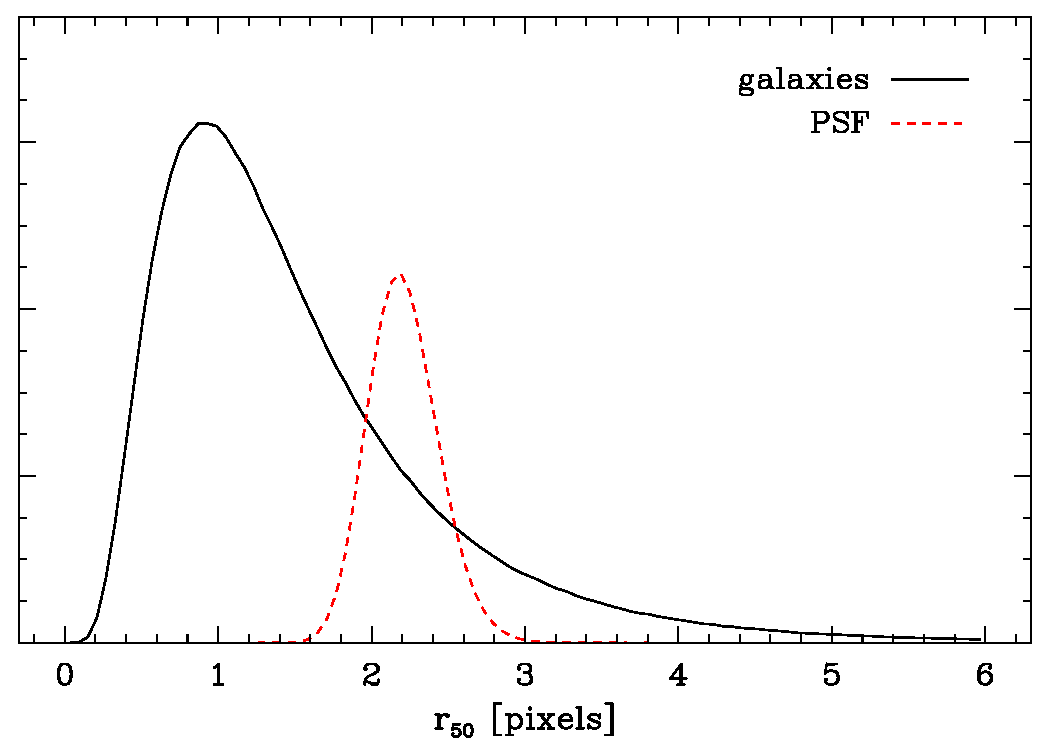
\includegraphics[scale=0.45]{sim-bd29-r50.eps}

    \caption{Distribution of half-light-radius \hlr\ in the Bulge+Disk simulations,
        for both galaxies and PSF.}

\label{fig:psimhlrcompare}
\end{figure}


We drew the PSF ellipticities from a distribution also designed to match that
measured in DES.  The DES PSF shape distribution is well fit by a double
Gaussian with width 0.18 in each dimension, but with different mean for $e_1$
and $e_2$.  We set the mean in $e_2$ to $0.007$, matching that in DES, but set
the mean in $e_1$ to zero as a control.

We designed the galaxy S/N distribution, shown in figure \ref{fig:s2n}, to
match the real DES galaxy catalog after a pre-selection of ``good galaxies''
\citep{DESSVShear}, but with no explicit S/N cut applied based on the model
fitting.  We adjusted the distribution slightly to give a distribution with
mode $\sim10$.  We sheared the galaxies with 1000 different randomly chosen values,
with amplitudes chosen uniformly in the range 0.01 to 0.08, and uniform random
orientations.

\begin{figure}
    \centering
    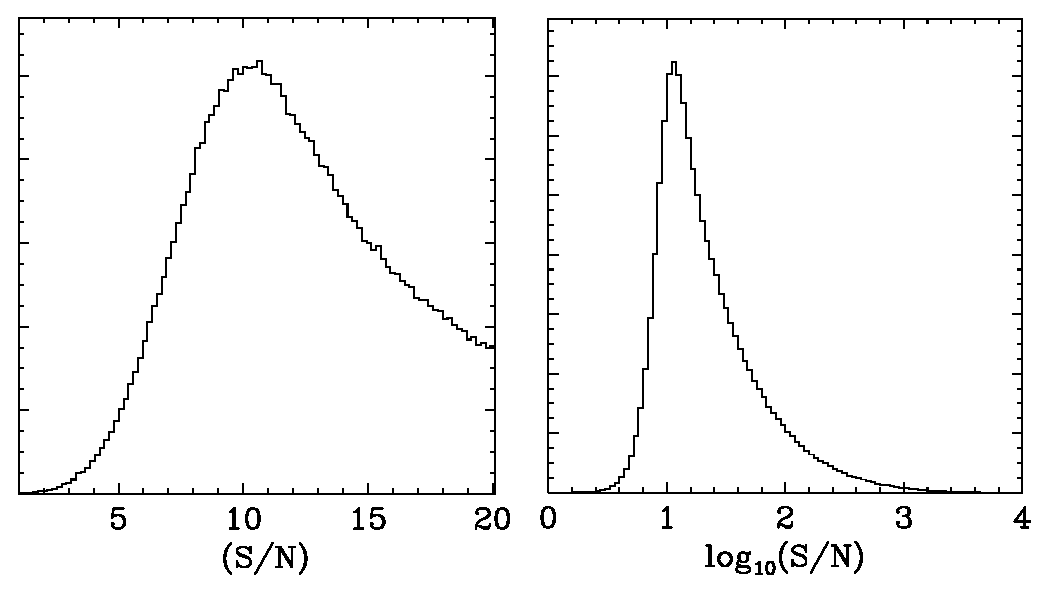
\includegraphics[scale=0.45]{s2n-bd29.eps}

    \caption{Distribution of S/N in the Bulge+Disk simulations. The
    left panel is a zoom-in around the mode.  The right panel is
the full distribution of $\log_{10}(S/N)$}

\label{fig:s2n}
\end{figure}


Ideally, the \mcalR\ measured for stars should be consistent with zero in the
mean, and thus not bias the ensemble shear estimate.  In order to test the
robustness of \mcal\ to stellar contamination, we included $\sim$\nsimNstarperc\ stars
in each simulation.  The stars were simply drawn as PSFs, with the same flux
distribution as used for the galaxies.  We refer to the simulations with
stars as ``BDStar''; the BD simulation is identical but with the stars
removed.

The Fourier transforms used to perform the \mcal\ convolutions cannot
accommodate missing data.  But in real data, ``bad pixels'' must be masked in
order to prevent biased measurements. For the FFTs, these masked pixels must be
replaced with some value that does not cause a bias in the statistics measured
on the transformed images.

We created another set of simulations, called ``BDMask'', in which we masked
parts of the data in order to mimic certain effects in real images.  In order
simulate these effects realistically, we chose a sample of real bit mask planes
used in Dark Energy Survey shear analysis \citep{DESSVShear}.  These include
masking of bad pixels, bad columns, and other image artifacts.   A random
sample of \nmasks\ masks were selected, removing those for which a masked pixel
fell within 4 pixels of the image center.  An example image and mask are shown
in figure \ref{fig:mask}.

\begin{figure}
    \centering
    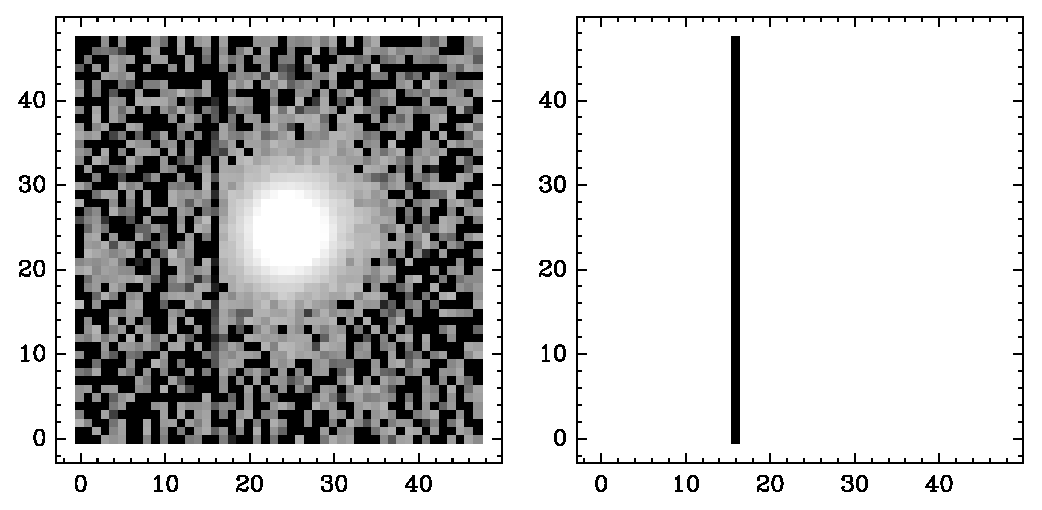
\includegraphics[scale=0.45]{DES2117+0126-bmask-021223.eps}

    \caption{Example DES image cutout and bitmask.  The vertical black stripe masks a
bad column. }

\label{fig:mask}
\end{figure}


\subsection{COSMOS Simulations}

We designed a second set of simulations to mimic the ``real-galaxy'' simulations
used in GREAT3 challenge \citep{great3}, using galaxy images draw from COSMOS
data.  We implemented two important changes.  First, we oriented the galaxies
randomly rather than placing them in pairs to cancel shape bias.  Using random
orientations avoids cancellation of systematics such as some selection effects
\citep{DESSVShear}.  Second, we used optical aberrations in the PSF designed to
match that seen in the Dark Energy Survey data \footnote{Aaron Roodman, private
communication}.  Similar to GREAT3, we varied the aberrations were varied as
Gaussian around a fiducial value. These root-mean-squared variations, in units
of waves in the Noll convention are given in table \ref{tab:aberr}.  We used a
Kolmogorov model for the atmospheric component, with mean FWHM = 0.9 arscec.
For this configuration there are significant variations in the PSF ellipticity,
but relatively little net ellipticity across the entire
ensemble of realizations.
The code used to generate these simulations began as a fork of the GREAT3
public code base, and is freely available
online\footnote{https://github.com/esheldon/egret}.

\begin{table}
    \centering
    \caption{Root-mean-squared variation for the aberrations in the optical model,
        in units of waves in the Noll convention, derived 
    from Dark Energy Survey data. \label{tab:aberr}}
    \begin{tabular}{ | l | l | }
        Zernike Component  & RMS Variation \\
        \hline
        Defocus & 0.13 \\
        Astigmatism in Y & 0.13 \\
        Astigmatism in X & 0.14 \\
        Coma in Y & 0.06 \\
        Coma in X & 0.06 \\
        Trefoil in Y & 0.05 \\
        Trefoil in X & 0.06 \\
        Spherical & 0.03 \\

    \end{tabular}
\end{table}

In figure \ref{fig:cosmos} we show the distribution of measured \snr\ for the
COSMOS simulations.  The mode of the distribution is somewhat higher than that
of the parametric simulations, about 12 instead of 10.  Also shown is the
distribution of the half-light-radius \hlr, measured
from the \sersic\ model fits distributed with the COSMOS catalog as part
of the GREAT3 challenge.  The mean \hlr\ for these simulations
is about $1.8 \pm 0.8$, somewhat smaller than the
log-normal $2.0 \pm 0.5$ for the parametric simulations, but with a tail to larger
size.


\begin{figure}
    \centering
    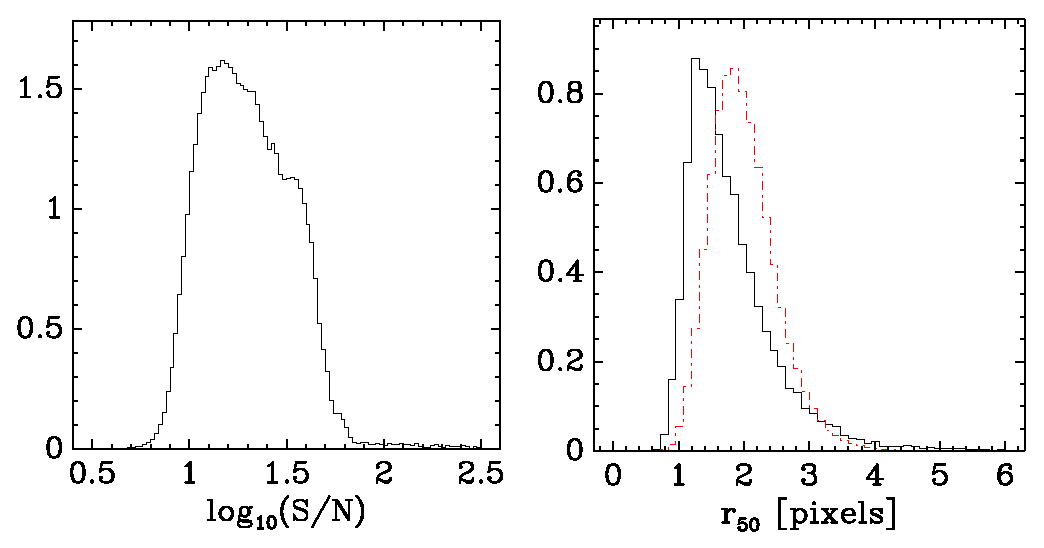
\includegraphics[scale=0.45]{mcal-v14s01-s2n-and-r50.eps}

    \caption{Distribution of properties in the COSMOS real galaxy simulations. The
    left panel contains the distribution of measured S/N, while the right panel contains
    the distribution of half-light-radius from the cosmos catalog for the input
    galaxies.  Overplotted as a red dashed line is the input half-light-radius
    for the bulge+disk simulations.}

\label{fig:cosmos}
\end{figure}





\begin{table*}
    \centering
    \caption{Description of the image simulations.  For the ``BD'' simulations,
        the Bulge and Disk had the same ellipticity and \hlr, but were offset
        uniformly up to \hlr, in a random direction.  The galaxy \hlr\ was drawn
        from a log-normal distribution with the specified mean and width, designed
        to roughly match the COSMOS galaxies.  The PSF ellipticity was
        drawn from a double Gaussian with the specified mean and width in each
        dimension.  The PSF FWHM was drawn from a log-normal distribution with
        the indicated mean and scatter, designed to roughly match
        that in DES data.  The ``BDStar'' simulation shared the
        same galaxy images with the ``BD'' simulation, but with additional star
        images included.  The ``BDMask'' simulation had masking for bad columns,
        bad pixels, drawn from DES data. For the RG
        simulation, real COSMOS images were used for the galaxies. For
        the PSF, a  Kolmogorov atmospheric turbulence model was used,
        with the indicated size,
        plus contributions from an optical model matched to DES. \label{tab:sims}}
    \begin{tabular}{ | l | c | c | c | c | c | c | c | c | c |}
        Sim          & Galaxy Model & Galaxy \hlr & PSF Model & PSF FWHM & PSF $e_1$      & PSF $e_2$           & \# Galaxies & \# Stars    & Masking   \\
                     &              & [pixels]    &           & [pixels]  &                &                     &             &             &  \\
        \hline
        BD           & Bulge+Disk   & \galrdist   & Moffat    & \psfrdist & \psfeonedist  &\psfetwodist   &  \nsimNgalFour   & None          & None      \\
        BDStar       & Bulge+Disk   & \galrdist   & Moffat    & \psfrdist & \psfeonedist  &\psfetwodist   &  \nsimNgalFour   & \nsimNStarFour & None      \\
        BDMask       & Bulge+Disk   & \galrdist   & Moffat    & \psfrdist & \psfeonedist  &\psfetwodist   &  \nsimNgalTwo   & None          & DES      \\
        %BDOLD           & Bulge+Disk   & Moffat    & \rpsfedist     &  \nsimNgal   & None        & None      \\
        %BDOLDStar       & Bulge+Disk   & Moffat    & \rpsfedist     &  \nsimNgal   & \nsimNStar  & None      \\
        %BDOLDEllip      & Bulge+Disk   & Moffat    & \psfedist  &  \nsimNgalTwo   & None        & None      \\
        %BDOLDEllipMask  & Bulge+Disk   & Moffat    & \psfedist  &  \nsimNgalTwo   & None        & DES       \\
        %BDMaskStar & Bulge+Disk   & Moffat    & \psfedist  &  \nsimNgal   & \nsimNStar  & DES      \\
        RG           & \cosmosname & \cosmosname & Kolm. + Optical & 3.40 + Optical  & Optical  & Optical  &  \nsimNgal   & None        & None      \\
    \end{tabular}
\end{table*}


\section{Results} \label{sec:detrendsim}

We fit the images with a single Gaussian galaxy model and Gaussian PSF model
using the \ngmix\ code\footnote{https://github.com/esheldon/ngmix}.  All \mcal\
operations were performed using the \texttt{metacal} module from \ngmix.

Naively using these grossly incorrect models resulted in a large model bias,
and large uncorrected PSF anisotropy.  In addition there was significant {\em
ordinary} noise bias at the low S/N levels used in the simulations.  We used
the \mcal\ procedure, coupled with the above correlated noise fixes,
to derive corrections for these biases.

We used a maximum likelihood fit, with smooth priors on all parameters to
produce a stable fit; for most simulations we had not a single failure. The
failures occurred when using the \detrend\ method, which included no correction
for correlated noise during the fitting process itself, which seems to have
destabilized a small number of the fits.  Even so, the failure rates for the
\detrend\ method was about 0.003\%.  These priors were not tuned to the true
galaxy parameters.  For the flux and size we deliberately used priors that were
wider than truth by 20\%.  For the ellipticity we used $\sigma=0.3$ instead of
the true $\sigma=0.2$.

\subsection{\mcal\ Responses}

R skewness -1.26 no fixnoise,  -0.30 with fixnoise

\begin{figure}
    \centering
    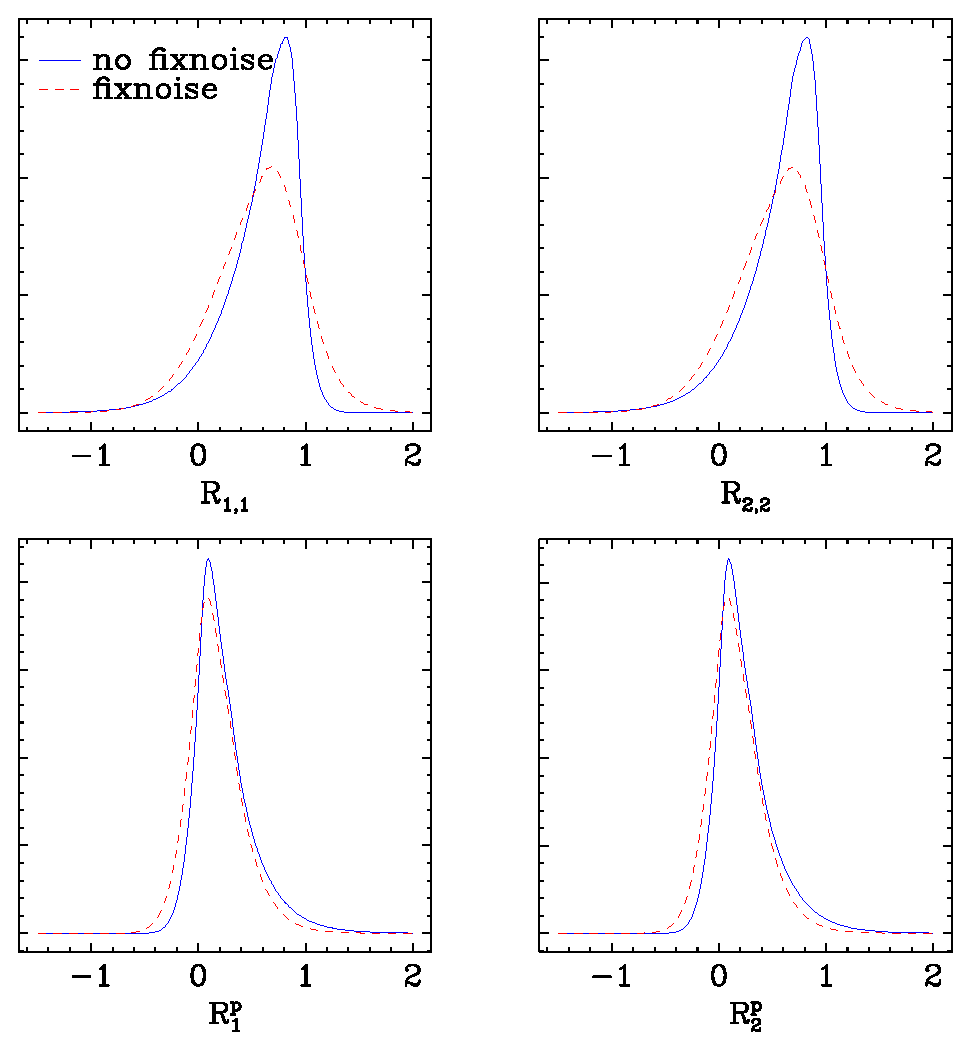
\includegraphics[scale=0.45]{mcal-v14s01-v14s02-compare-R.eps}

    \caption{Distribution of \mcal\ responses for the real galaxy
    simulation, with and without the ``\fixnoise'' corrections
    for correlated noise.  For the \fixnoise\ correction, we
    added a convolved, sheared noise field designed to statistically
    cancel the effects of correlated noise.  The extra noise
    broadens the distribution, but the correction results in a more symmetric
    distribution.  The top panels represent the multiplicative
    response \mcalR\ and the bottom panels represent the PSF response \mcalRpsf.} 

\label{fig:Rdist}
\end{figure}


\subsection{Shear Recovery}


In table \ref{tab:results} we show for shear recovery in our simulations, with
and without applying correlated noise corrections.  Without correction, the
multiplicative bias $m$ is of order 0.1 for all simulations.  For simulations
with a net PSF anisotropy, we also found a significant remaining additive bias.

\begin{table*}
    \centering
    \caption{\Mcal\ results for each image simulation described in
        \S \ref{sec:sims} and table \ref{tab:sims}.  A single Gaussian was fit
    to both galaxy and PSF, resulting in significant multiplicative 
    bias $m$ and additive biases $c$ before applying the \mcal\ response
    terms. With \mcal, no multiplicative bias was detected in any case. 
    Some remaining additive bias in $g_2$ was detected, due to the use of
    intentionally poor psf correction, but \mcal\ reduced the
    bias by a factor of 13.
    Stellar contamination at the level of \nsimNstarperc\ increases
    the noise in the recovered shear by $\sim$5\% but does not introduce 
    a significant bias.  Replacing bad pixels and columns with the best fit model
    did not introduce any detected bias.
    \label{tab:results}}
    \begin{tabular}{ |l|  c|c|c|  c|c|c|}
        \hline
        & \multicolumn{3}{c}{Maximum Likelihood}                    & \multicolumn{3}{c}{\Mcal} \\
        Sim    & $m$         & $c_1$            & $c_2$             & $m$               & $c_1$            & $c_2$ \\
               & $[10^{-3}]$ & $[10^{-4}]$      & $[10^{-4}]$       & $[10^{-3}]$       & $[10^{-4}]$      & $[10^{-4}]$ \\
        \hline
        BD     & $-496$      & $+0.05 \pm 0.07$ & $15.21 \pm 0.07$  & $-0.27 \pm 0.34$  & $+0.00 \pm 0.17$ & $+1.12 \pm 0.17$  \\
        BDStar & $-541$      & $+0.1 \pm 0.1$   & $18.3 \pm 0.1$    & $-0.21 \pm 0.36$  & $+0.03 \pm 0.18$ & $+1.21 \pm 0.18$  \\
        BDMask & $-496$      & $+0.09 \pm 0.10$ & $15.07 \pm 0.10$  & $-0.60 \pm 0.46$  & $-0.17 \pm 0.23$ & $+0.73 \pm 0.23$  \\
        RG     & $-436$      & $-0.2 \pm 0.2$   & $~~0.3 \pm 0.2$   & $+0.53 \pm 0.58$  & $-0.42 \pm 0.29$ & $+0.59 \pm 0.29$ \\
        %& \multicolumn{3}{c}{Maximum Likelihood}                     & \multicolumn{3}{c}{\Mcal\ Uncorrected}            & \multicolumn{3}{c}{\Mcal\ Corrected} \\
        %Sim    & $m$              & $c_1$         & $c_2$            & $m$             & $c_1$          & $c_2$          & $m$            & $c_1$           & $c_2$ \\
        %       & $[10^{-3}]$      & $[10^{-4}]$   & $[10^{-4}]$      & $[10^{-3}]$     & $[10^{-4}]$    & $[10^{-4}]$    & $[10^{-3}]$    & $[10^{-4}]$     & $[10^{-4}]$ \\
        %\hline
        %BD     & $-495.6 \pm 0.2$ & $+0.1 \pm 0.1$ & $15.1 \pm 0.1$  & $104.5 \pm 0.5$ & $-0.3 \pm 0.2$ & $-5.6 \pm 0.2$ & $-0.4 \pm 0.5$  & $+0.0 \pm 0.2$ & $+0.9 \pm 0.2$  \\
        %BDStar & $-541.1 \pm 0.2$ & $+0.1 \pm 0.1$ & $18.3 \pm 0.1$  & --              & --             & --             & $-0.2 \pm 0.5$  & $+0.0 \pm 0.2$ & $+1.0 \pm 0.2$  \\
        %RG     & $-435.6 \pm 0.3$ & $-0.2 \pm 0.2$ & $~~0.3 \pm 0.2$ & $125.3 \pm 0.5$ & $-0.3 \pm 0.3$ & $+0.0 \pm 0.3$ & $+0.5 \pm 0.6$  & $-0.4 \pm 0.3$ & $+0.6 \pm 0.3$ \\
    \end{tabular}
\end{table*}

XXX describe both kinds of corrections

After applying correlated noise corrections, we found the multiplicative bias
to be consistent with zero within errors for the parameteric simulations. For
the real galaxy RG simulation we detect remaining multiplicative bias of
approximately \rgbias.  For the BDEllip parameteric simulations, which have a
net psf anisotropy, we still detected a small remaining additive bias, but it
was reduced by a factor of five in amplitied, as compared to results without
correlated noise corrections.

\subsection{Stellar Contamination} \label{sec:stars}

As indicated in table \ref{tab:sims}, for the ``Star'' type simulations, we
included an additional \nsimNStarTwo\ stellar objects, \nsimNstarperc, drawn simply as a PSF
with noise added.  The galaxy images were the same as used in the BD
simulation.  The results are shown in table \ref{tab:results} for the BDStar
type simulation.  We did not detect any multiplicative bias due to
including the stars.

\Mcal\ is robust to stellar contamination as long as the PSF is well
known.  Images consistent with a PSF will not, in the mean, respond to the shear
applied during the \mcal\ process.  They also yield zero average shape, as
long as the PSF correction is sufficiently accurate:
\begin{align}
    \gamma &= \frac{ \langle e_{gal} \rangle + \langle e_{star} \rangle - \langle R^p_{gal} + R^p_{star} \rangle \langle e^p \rangle }{ \langle R^{gal} \rangle + \langle R^{star} \rangle}.
\end{align}
In figure \ref{fig:Rstars} we show the measured response \mcalR\ for stars
and galaxies.  Indeed we see that \mcalR\ is noisy but conistent with
zero for the stars.

\begin{figure}
    \centering
    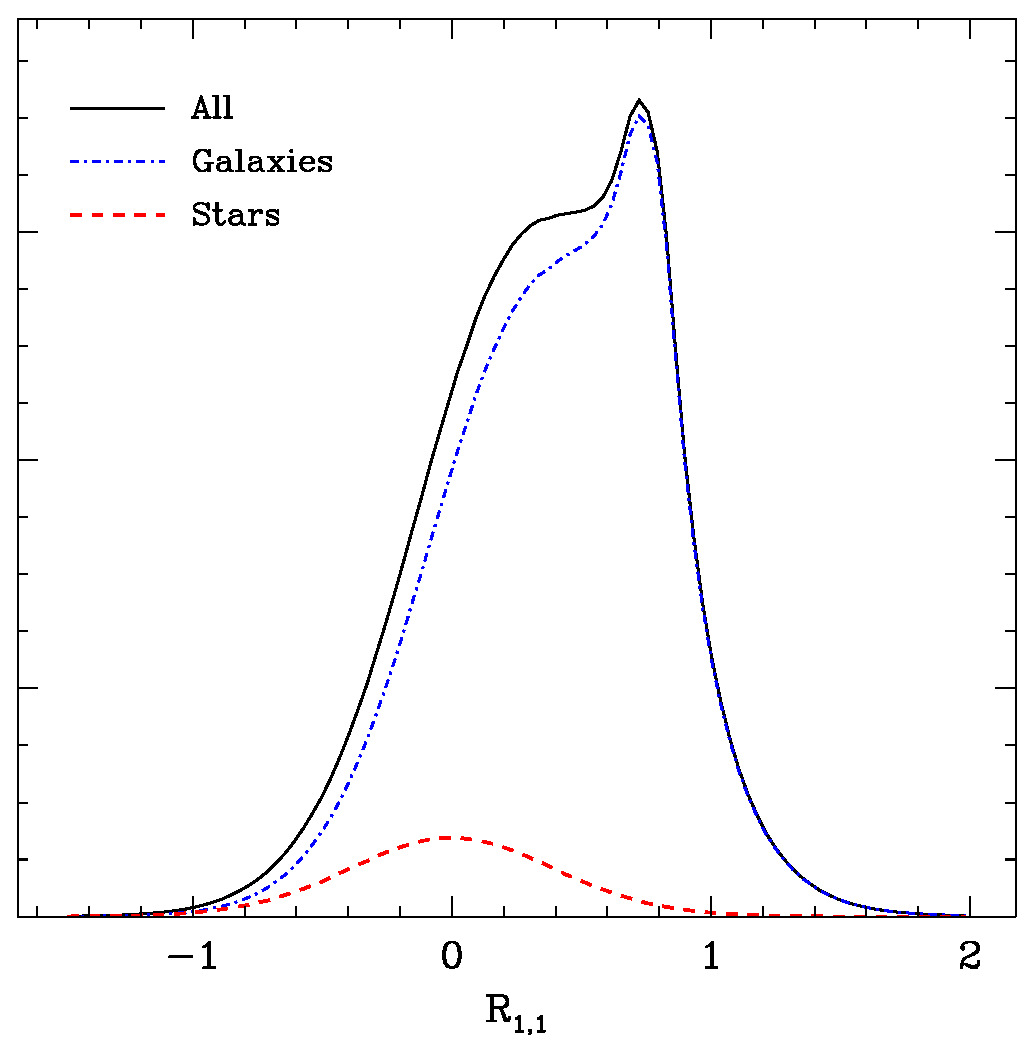
\includegraphics[scale=0.45]{R-bd29-bd29stars.eps}

    \caption{Distribution of \mcal\ responses for galaxies and stars in
    the BDStar simulation.  Stars have mean response close to zero,
    and thus do not bias the overall shear calibration.}

\label{fig:Rstars}
\end{figure}

We used a very poor psf correction, based on a single gaussian, yet we did
not detect any significant additional bias.  However, including \nsimNstarperc\ stars
did increase the bias but about 5\%.

If the additional variance is tolerable, it may be useful to include stars in a
shear analysis.  Attempting to remove faint stars from a sample is a noisy
procedure, likely to induce selection effects: for example stars that are
included in the sample after a size cut will have fluctuated to larger size due
to noise, and will also likely have fluctuated to higher response \mcalR,
biasing the recovered shear.

For accurate interpretation of the signal, it is still important that any
redshift estimates for the stars are consistent with zero, in the mean.  Stars
could also be down-weighted using an appropriate weighting scheme.  We can
rewrite equation \ref{eq:basicestimator} as
\begin{align}
    \langle \gamma \rangle &= \frac{ \sum E }{\sum \mbox{\mcalR}} = \frac{ \sum \mbox{\mcalR}^{true} \gamma }{\sum \mbox{\mcalR}},
\end{align}
which would look like a weighted average if the measured \mcalR\ were equal to
the true response $\mbox{\mcalR}^{true}$.  The measured \mcalR\ could be used
to weight the redshift estimates as well, although one must be careful as the
\mcalR\ are not strictly positive.

\subsection{Masking Effects} \label{sec:masking}

In order to perform the Fourier transforms used for the \mcal\ convolutions, we
must replace any missing data due to masked pixel values.  In particular we
wish to avoid any artifacts in the transformed images that would mimic an
additional ``response'' to the applied \mcal\ shear.

As an baseline extreme case, we replaced the masked pixels simply with noise.
This resulted in few percent calibration biases.

A better alternative is to replace the missing data with the result of a model
fit.  We performed an initial maximum likelihood fit, before performing any
\mcal\ operations, and replaced the masked data with the value from the PSF
convolved model.  We used a Gaussian model for both PSF and Galaxy, which is a
poor representation of the data; we consider this a worst case scenario as a
model replacement. 

The results using the model replacement method are shown in table
\ref{tab:results} for the BDEllipMask simulation.  The measured bias did not
change significantly compared to the measurements on BDEllip, which is the
unmasked version of this simulation.


\subsection{Selection Effects} \label{sec:selection}

There are two main types of selection: detection effects and ordinary selection
effects.  Detection effects occur when placing a detection threshold on a
quantity that correlates with galaxy shape. One example is \snr: cutting to
objects greater than some value of \snr\ will preferentially remove galaxies
with higher ellipticity, and thus reduce the inferred shear.  Ordinary
selection on an initially unbiased detected sample can induce additional bias
via the same mechanism.

Determining detection effects may require prior information about the
properties of the galaxies in the sample, including those galaxies that do not
exceed the detection threshold.  Ordinary selection effects can in principle be
determined without prior information if the initial detections were unbiased,
but unbiased detection of faint galaxies is unlikely to be feasible.

To test selection effects, we made a series of cuts on S/N in the BD
simulation.  We used the ``round'' \snr\ definition in order to avoid the first
order effect \citep{DESSVShear}.  We found the magnitude of the multiplicative
bias increased monotonically with the cut on \snr, reaching a bias of $\sim
-2.5 \times 10^{-3}$ for $S/N > 20$.  This bias is larger than the requirements
for future surveys.

The detection bias could potentially be even larger than what we found, since
the cut would be applied to a distribution of intrinsic \snr\ that is
approximately a power law shape, rather than one with a cutoff, as we had in
our simulations. We will explore how to miticate these important selection
effects in a future work.

\begin{comment}
As indicated in table \ref{tab:selresults},
these cuts lead to a monotonic change in the recovered shear, with a few
tenths of a percent bias for a $S/N > 20$ cut.

\begin{table*}
    \centering
    \caption{\Mcal\ results when applying selections on the signal-to-noise ratio (S/N) to the BD simulations. Selections
    were applied to an initially unbiased sample; i.e. no {\em detection}
    bias was present in the sample. \label{tab:selresults}}
    \begin{tabular}{ |l| r|r|r|  r|r|r|}
        \hline
        & \multicolumn{3}{c}{Uncorrected for Selection} & \multicolumn{3}{c}{Corrected for Selection} \\
        Selection & $m \times 10{^3} $ & $c_1 \times 10^4$ & $c_2 \times 10^4$ & $m \times 10^{3}$ & $c_1 \times 10^4$ & $c_2 \times 10^4$ \\
        \hline
        %$(S/N) > 5$    & $3.0 \pm 4.4$ & $-0.3 \pm 0.2$ & $0.2 \pm 0.2$ & $3.3 \pm 4.4$ & $-0.3 \pm 0.2$ & $0.2 \pm 0.2$  \\
        $(S/N) > 7.5$  & $-0.7 \pm 0.4$ & $-0.3 \pm 0.2$ & $0.2 \pm 0.2$ & $-0.6 \pm 0.4$ & $-0.3 \pm 0.2$ & $0.2 \pm 0.2$  \\
        $(S/N) > 10$   & $-1.5 \pm 0.5$ & $-0.3 \pm 0.2$ & $0.2 \pm 0.2$ & $-1.0 \pm 0.5$ & $-0.3 \pm 0.2$ & $0.2 \pm 0.2$  \\
        $(S/N) > 15$   & $-2.3 \pm 0.5$ & $0.0 \pm 0.3$ & $0.0 \pm 0.3$ & $-0.9 \pm 0.5$ & $0.0 \pm 0.3$ & $0.0 \pm 0.3$  \\
        $(S/N) > 20$   & $-2.7 \pm 0.6$ & $-0.3 \pm 0.3$ & $-0.2\pm 0.3$ & $-0.9 \pm 0.6$ & $-0.3 \pm 0.3$ & $-0.2 \pm 0.3$  \\
    \end{tabular}
\end{table*}

We implemented a simple correction based on our \mcal\ measurements.  We
sheared the population of ellipticities with a fake shear using the measured
responses \mcalR, and estimated the shear using our \mcal\ mechanism before and
after selection.  We then used the ratio of these numbers as a correction
factor.  We sow the results in table \ref{tab:selresults} in the ``Corrected
for Selection'' column.  This simple correction reduced the bias approximately
$10^{-3}$ in all cases.

In real data, a simple correction scheme like the above will probably require
prior information.  One approach would be to take deep imaging data and add
noise such that the distribution of $S/N$ for the galaxy sample is similar to a
shallower data set.  The noisy ellipticity measurements could then be sheared
artificially and selected as above to derive a correction.  Multiple noise
realizations could be used to increase the precision of the correction.
\end{comment}


\section{Bias in GREAT3 Simulations}

Relatively little bias was seen by \cite{HuffMcal} using the GREAT3 simulations
\citep{great3}.  We checked that our code used to perform the metacal
procedures gives identical results to that used in \cite{HuffMcal}, so this is
most likely not a software error.  Rather, we suspect that the higher S/N and
better modeling used in \cite{HuffMcal} resulted in reduced bias.

The correlated noise effect scales with the square of the noise, and the
simulations used for GREAT3 contain significantly higher S/N galaxies than the
simulations used in this work.  Indeed, we found the correlated noise was still
detectable in simulations we ran with similar properties to GREAT3, but with
correlated noise bias at the 1-2\% level rather than the 12\% we saw in our RG
simulations.  We also ran the re-gaussianization code on our simulations, and
did see a bias, but about a factor of two lower than we saw for our
intentionally bad Gaussian PSF and Galaxy models.

Another important difference between the GREAT3 sims and our sims is that
GREAT3 galaxies were generated in pairs, rotated by 90 degrees with respect to
a one another, in order to cancel shape noise.  However, we ran one of our
simulations in such a configuration and saw the same level of correlated noise
bias.  This is not surprising; the correlated noise effect adds coherently to
the response, and should not cancel due to such imposed symmetries in the
underlying galaxy population.

\section*{Acknowledgments}

ES is supported by DOE grant DE-AC02-98CH10886.

We thank Aaron Roodman for providing the variation of the optical aberrations
measured in DES data.  Thanks to Mike Jarvis for guidance on use of the GALSIM
package, especially concerning use of the isotropization and whitening features.


\appendix

\section{Additional Correction Methods} \label{sec:altcorr}

\subsection{Correction using GALSIM}

With guidance from the GALSIM developers, we attempted to use the GALSIM noise
isotropization and whitening functionality to correct the correlated noise.
Isotropization enforces four fold symmetry, introducing minimal extra noise,
while whitening completely whitens the image, introducing significant extra
noise.  However, neither of these methods improved the shear recovery in our
simulations.  It may be that some aspects of the \mcal\ procedure invalidate
the assumptions behind these correction methods.


\subsection{Detrending the Correlated Noise Bias} \label{sec:detrend}

We expect the bias in \mcalR\ due to correlated noise to scale with the square
of the noise in the image $n^2$ (see \S \ref{sec:scaling}).  We can add a small
amount of noise to the image such that $n \rightarrow n + \Delta n$.  If we
then run the new image through the \mcal\ process, we can measure
$R^{\mathrm{before}}$, a response that will include correlated noise effects.
We can write this observed response as
\begin{align}\label{eq:Rbefore}
    R_o^{\mathrm{before}} &= R + A (n + \Delta n)^2 \nonumber \\
       &\simeq R + A n^2 + 2 A n \Delta n
\end{align}
%&\simeq R + A n^2 + \frac{\partial (An^2)}{\partial n} \Delta n + ... \nonumber \\
where we have dropped terms of order $(\Delta n)^2$ and higher.  In equation
\ref{eq:Rbefore}, \mcalR\ is the response at noise $n+\Delta n$ in the absence
of correlated noise.  

We can also add identical noise {\em after} the original image  has been run
through \mcal, and measure $R^{\mathrm{after}}$.  The response when adding
noise after \mcal\ does not suffer any additional bias due to correlated noise:
\begin{align}
    R_o^{\mathrm{after}} &= R + A n^2.
\end{align}
The difference between these responses is then 
\begin{align}
    \Delta R &\equiv R_o^{\mathrm{before}} - R_o^{\mathrm{after}}  \nonumber \\
             &\simeq 2 A n \Delta n.
\end{align}

We propose the following procedure to correct for correlated noise:
\begin{enumerate}
    \item Calculate $\Delta R$ for a series of noise offsets $\Delta n$.
    \item Average $\Delta R$ over all objects for each noise offset.
    \item Perform a linear fit to $\Delta R$ vs. $2 n \Delta n$ to find the 
        coefficient $A$.
    \item Apply a mean correction for correlated noise given by
        \begin{align}
            \mbox{\mcalRnoise} & \simeq A n^2.
        \end{align}
        with a similar correction for \mcalRpsf.
\end{enumerate}
If the noise varies between observations, we can apply a 
correction based on the mean variance $A
\langle n^2 \rangle$.

\subsubsection{Measurements of the \detrend\ Parameters}

For the \detrend\ method, we measured $\Delta R$ vs $2 n \Delta n$ to find the
coefficient $A$.  In figure \ref{fig:detrend}, we show this fit for the RG
simulation.  The trend is well-fit by a linear model, as expected, with a slope
$A \simeq $\Aslope, implying a correction $A n^2 \simeq$ \Rcorr\ for this
simulation.

\begin{figure}
    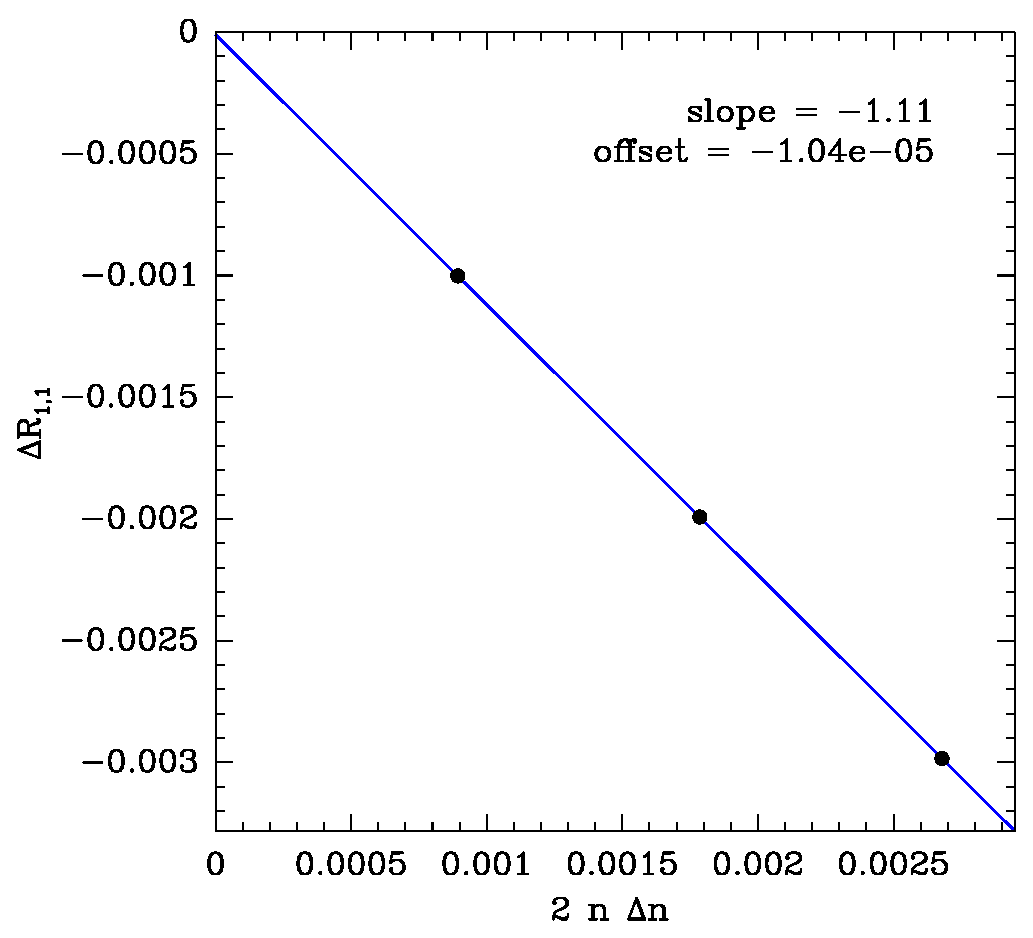
\includegraphics[scale=0.45]{mcal-v14s01-Rnoise-detrend-R11.eps}

    \caption{Trend of $\Delta R_{1,1}$ with $2 n \Delta n$ for the
        real galaxy simulation.   $n$ is the
    original noise level and $\Delta n$ is the additional noise added.  The
    trend is linear as predicted.}

\label{fig:detrend}
\end{figure}




\subsubsection{Using a Random Subset To Calculate \Detrend\ Corrections}

Measuring the \detrend\ parameters requires extra computations, at least a
factor of three to fit the linear parameters given in \S \ref{sec:detrend}, and
a factor of four if an additional point is used to check for possible
non-linearity. These extra computations could be expensive for large surveys.  

However, the \detrend\ parameters are more precisely measured than the shear
itself.  Here we explore the precision of the recovered shear using smaller
subsets of the object catalog to measure the \detrend\ parameters, and
applying the corrections to the full sample.  In Table \ref{tab:subsets}
we show the shear recovery parameters for various subset sizes, for the
BD simulation described in \S \ref{sec:detrendsim}

\begin{table*}
    \centering
    \caption{Additional variance in the recovered shear 
        using different sized subsets to
        estimate the detrending corrections.  Values were obtained
        from 100 bootstrap samples. \label{tab:subsets}}
    \begin{tabular}{| c | c |}
        Subset Size & Extra Error \\
        \hline
        1\% & 4.4\% \\
        5\% & 0.8\% \\
        10\% & 0.3\% \\
    \end{tabular}
\end{table*}
%        1\% & 30\% \\
%        5\% & 13\% \\
%        10\% & 8\% \\


We find that a relatively small sample can be used to determine the correlated
noise correction.  Calculating the detrending terms for 10\% of the sample
leads to only 0.3\% extra variance in the recovered shear, and using 1\% of
galaxies leads to only 4.4\% increase in variance.

To calculate these numbers we have assumed the extra uncertainty is added
quadratically with the uncertainty measured using all galaxies to estimate the
\detrend\ parameters; e.g for the first row, we have added approximately 30\%
quadratically with the measured uncertainty, resulting in a net increase of
4.4\%.

It is important to use a truly random subset of the population to determine the
corrections, including a fair sample of stars and other contaminants, and a
representative amount of pixel level masking.  If a particular aggregate shear
measurement involves a selection, this selection must also be applied to the
random subset.

\subsubsection{Performance of the \detrend\ method}

We found this method did not work as well as the \fixnoise\ method
described in \S \ref{sec:fixnoise}.  We detected a remaining bias
of $m \sim 2 \times 10^{-3}$ in both the BD and RG simulations.

\subsection{Simulating Models}

In this method, we generated model images with the correct noise level corresponding
to each real imag.  We then measured the response of the noise due to the
convolutions and shears used in \mcal, with noise added before and
after the \mcal\ procedure.

The measurement with correlated noise will be the sum of the response
without correlated noise plus the response of the correlated noise field
\begin{equation}
    \mbox{\mcalRnoisemodel} = \mbox{\mcalRmodel} + \mbox{\mcalRnoise}
\end{equation}
This measurement is quite noisy for a single galaxy, but we
can estimate the mean correlated noise response for an ensemble
of galaxies
\begin{equation}
    \langle \mbox{\mcalRnoise} \rangle = \langle \mbox{\mcalRnoisemodel} \rangle - \langle \mbox{\mcalRmodel} \rangle.
\end{equation}
Each entry used in this average corresponds to the best fit model
and noise properties for a galaxy in the sample.

The response \mcalRnoise\ can be subtracted to recover an estimate of the mean
response without correlated noise
\begin{equation}
    \langle \mbox{\mcalR} \rangle = \langle \mbox{\mcalRo} \rangle - \langle \mbox{\mcalRnoise} \rangle.
\end{equation}
These responses will be noisier than the original images, due to the
independent noise in both \mcalRo\ and \mcalRnoise.  To increase
precision, the procedure can be repeated for different noise fields
and averaged, at the cost of increased computation time.

We found this method performed poorly.  We detected a remaining bias of  $m
\sim 4 \times 10^{-3}$ in both the BD and RG simulations.


\bibliographystyle{mn2e}
% Bib database
\bibliography{apj-jour,astroref}

\end{document}

